\documentclass[11pt,a4paper]{article}

\usepackage[utf8]{inputenc}
\usepackage[T1]{fontenc}
\usepackage{amsmath,amssymb,amsthm}
\usepackage{mathtools}
\usepackage{booktabs}
\usepackage{hyperref}
\usepackage{cleveref}
\usepackage{listings}
\usepackage{xcolor}
\usepackage{tikz}
\usetikzlibrary{positioning,arrows.meta,shapes.geometric,calc}
\usepackage[margin=1in]{geometry}
\usepackage{natbib}
\usepackage{enumitem}

% Theorem environments
\newtheorem{theorem}{Theorem}[section]

% Math operators
\DeclareMathOperator{\Aut}{Aut}
\DeclareMathOperator{\SO}{SO}
\DeclareMathOperator{\SU}{SU}
\DeclareMathOperator{\GL}{GL}
\DeclareMathOperator{\PG}{PG}
\DeclareMathOperator{\Ima}{Im}
\newcommand{\Oct}{\mathbb{O}}
\newcommand{\Real}{\mathbb{R}}
\newcommand{\Comp}{\mathbb{C}}
\newcommand{\Quat}{\mathbb{H}}
\newcommand{\Sed}{\mathbb{S}}

% Code listing style
\definecolor{codebg}{gray}{0.96}
\definecolor{codegreen}{rgb}{0.0,0.5,0.0}
\definecolor{codegray}{rgb}{0.5,0.5,0.5}
\lstdefinestyle{python}{
  backgroundcolor=\color{codebg},
  basicstyle=\ttfamily\small,
  keywordstyle=\color{blue},
  commentstyle=\color{codegreen},
  stringstyle=\color{red!70!black},
  language=Python,
  frame=single,
  framerule=0.4pt,
  xleftmargin=1em,
  xrightmargin=1em,
  breaklines=true,
  showstringspaces=false,
}

% Epistemic honesty environment
\newenvironment{epistemicnote}{%
  \medskip\noindent\textbf{Epistemic honesty note.}\itshape\space
}{%
  \medskip
}

% Pseudocode label
\newcommand{\pseudocodelabel}{\hfill\textit{(pseudocode; not yet implemented)}}

\title{Octonionic Computation as a Substrate for\\Geometric Reasoning in Machine Learning}
\author{Antonio Escalera}
\date{March 2026\\[0.5em]\normalsize Working Draft}

\begin{document}
\maketitle

\begin{abstract}
We propose that the octonions~($\Oct$), as the largest normed division algebra over the reals, constitute an optimal primitive substrate for encoding knowledge and performing reasoning in machine learning systems. This claim rests on a convergence of algebraic, geometric, and information-theoretic arguments: octonions maximize representational density per algebraic unit among division algebras, their non-associativity naturally encodes context-dependence, and the division algebra property guarantees that all transformations are invertible, a prerequisite for reasoning about missing or uncertain information.

We describe an architecture for a system (the ``Octonionic Reasoning Engine'' or ORE) that ingests heterogeneous real-time data streams, encodes them into octonionic representations whose dimensional semantics are learned rather than prescribed, and reasons by applying sequences of geometric transformations within and between octonionic spaces. We further argue that the natural geometry of the octonionic state space is hyperbolic rather than flat: the exponential volume growth of hyperbolic space provides the correct scaling for hierarchical knowledge representation, gives the ``geometry of absence'' (uncertainty about missing information) a rigorous formulation, and establishes a natural correspondence between an octonion's real/imaginary decomposition and the timelike/spacelike split of hyperbolic space in the hyperboloid model.

We argue this combined octonionic-hyperbolic approach enables a form of deep geometric reasoning that is fundamentally more expressive per parameter than real-valued, complex, or quaternionic alternatives, and that the algebraic ceiling imposed by Hurwitz's theorem makes octonions the natural terminus of this line of inquiry.
\end{abstract}

\tableofcontents
\newpage

%% ====================================================================
\section{Mathematical Foundations}
\label{sec:foundations}
%% ====================================================================

\subsection{The Normed Division Algebras}
\label{sec:nda}

The central mathematical result underlying this work is a classification theorem from abstract algebra.

\begin{theorem}[Hurwitz, 1898]
The only normed division algebras over~$\Real$ are the reals~($\Real$, dim~1), the complex numbers~($\Comp$, dim~2), the quaternions~($\Quat$, dim~4), and the octonions~($\Oct$, dim~8).
\end{theorem}

\begin{table}[ht]
\centering
\caption{The four normed division algebras.}
\label{tab:nda}
\begin{tabular}{@{}lcccccc@{}}
\toprule
Algebra & Symbol & Dim & Associative & Commutative & Division & Zero divisors \\
\midrule
Reals       & $\Real$ & 1 & Yes & Yes & Yes & None \\
Complex     & $\Comp$ & 2 & Yes & Yes & Yes & None \\
Quaternions & $\Quat$ & 4 & Yes & No  & Yes & None \\
Octonions   & $\Oct$  & 8 & No  & No  & Yes & None \\
\bottomrule
\end{tabular}
\end{table}

Each step in the Cayley--Dickson construction doubles the dimension while sacrificing an algebraic property: $\Comp$~loses ordering, $\Quat$~loses commutativity, $\Oct$~loses associativity. Beyond octonions, the sedenions ($\Sed$, dim~16) and all subsequent algebras lose the division property, meaning they contain zero divisors: non-zero elements whose product is zero.

The presence of zero divisors has a direct consequence for computation. If $ab = 0$ where both $a \neq 0$ and $b \neq 0$, then the transformation ``multiply by~$a$'' irreversibly annihilates information carried by~$b$. This renders sedenions and beyond fundamentally unsuitable for any architecture requiring reversible reasoning (\cref{sec:reversibility}).

Hurwitz's theorem is a proven classification, not a conjecture. No 16-dimensional normed division algebra can exist. Octonions are the terminal object in this sequence.

\subsection{Octonionic Algebra}
\label{sec:octalgebra}

An octonion $x \in \Oct$ is written:
\begin{equation}
x = x_0 + x_1 e_1 + x_2 e_2 + x_3 e_3 + x_4 e_4 + x_5 e_5 + x_6 e_6 + x_7 e_7,
\end{equation}
where $x_0, \ldots, x_7 \in \Real$ and $e_1, \ldots, e_7$ are imaginary basis units. Multiplication is defined by the \textbf{Fano plane}, a combinatorial structure encoding 7 oriented triples (see \cref{app:fano}). Each line of the Fano plane defines a quaternionic subalgebra; the full multiplication table is governed by these triples.

Key properties:
\begin{itemize}[nosep]
  \item \textbf{Alternativity:} $(xx)y = x(xy)$ and $(xy)y = x(yy)$ hold for all octonions, even though $(xy)z \neq x(yz)$ in general. The subalgebra generated by any two octonions is always associative (Artin's theorem).
  \item \textbf{Norm preservation:} $\lvert xy \rvert = \lvert x \rvert \lvert y \rvert$, ensuring the product of unit octonions is a unit octonion.
  \item \textbf{Unique inverses:} Every non-zero octonion has a unique inverse $x^{-1} = \bar{x} / \lvert x \rvert^2$.
  \item \textbf{The associator} $[x,y,z] = (xy)z - x(yz)$ is a totally antisymmetric trilinear form, and is itself a geometrically meaningful object.
\end{itemize}

In this implementation, multiplication is computed as a single \texttt{torch.einsum} call over the $8 \times 8 \times 8$ structure constants tensor~$C_{ijk}$, where $(a \cdot b)_k = \sum_{i,j} C_{ijk}\, a_i\, b_j$. This approach fully vectorizes over batch dimensions. See \texttt{src/octonion/\_multiplication.py}.

\subsection{The Automorphism Group \texorpdfstring{$G_2$}{G2}}
\label{sec:g2}

The automorphism group of~$\Oct$ is the exceptional Lie group $G_2$, a 14-dimensional compact Lie group that acts on the 7-dimensional space of imaginary octonions ($\Ima\Oct \cong \Real^7$) while preserving the octonionic multiplication structure.

$G_2$ provides a natural symmetry group for learned transformations. A model that learns to operate within~$G_2$ is learning transformations that respect the full algebraic structure of the octonions, analogous to how $\SO(3)$ transformations in quaternionic models respect 3D rotational geometry, but with substantially richer structure.

$G_2$ sits inside $\SO(7)$ (the 21-dimensional rotation group of~$\Real^7$) as a proper subgroup. $G_2$ transformations are rotations that additionally preserve the octonionic product. This constraint imposes geometric coherence on learned transformations, reducing the parameter space from 21 to 14 dimensions while retaining all algebra-preserving degrees of freedom.

\subsection{The Fano Plane as Computational Architecture}
\label{sec:fano}

The Fano plane, the finite projective plane $\PG(2,2)$, encodes the octonionic multiplication table. It has 7 points, 7 lines, and its symmetry group is $\GL(3, \mathbb{F}_2)$ of order~168.

Each line of the Fano plane defines a quaternionic subalgebra of~$\Oct$. There are exactly 7 such subalgebras, and they overlap: each imaginary unit belongs to exactly 3 subalgebras. This structure has several consequences:
\begin{itemize}[nosep]
  \item Any two imaginary octonions generate an associative (quaternionic) subalgebra.
  \item Computation within a single subalgebra is fully associative, and thus directly analogous to quaternionic ML.
  \item Non-associativity arises only when computing across subalgebras, i.e., when integrating information from distinct quaternionic subspaces.
\end{itemize}

The octonion therefore naturally decomposes into 7 overlapping quaternionic channels. Local computation within a channel is associative and well-understood; cross-channel computation is non-associative and introduces the richer geometric structure unique to~$\Oct$. This decomposition is central to the architecture described in \cref{sec:architecture}.

%% ====================================================================
\section{The Reversibility Thesis}
\label{sec:reversibility}
%% ====================================================================

\subsection{Reversibility as a Requirement for Reasoning Under Uncertainty}

Consider the problem of reasoning about missing information. If a system has processed a data stream and built an internal representation, and then encounters a gap (missing data, a corrupted signal, an unobserved event), it must:
\begin{enumerate}[nosep]
  \item Identify that information is missing (detect the gap).
  \item Characterize what kind of information is missing (bound the gap).
  \item Generate candidate hypotheses for the missing content (fill the gap).
  \item Evaluate those hypotheses against the world model (test the gap).
\end{enumerate}

Steps 3 and 4 require running the model's transformations in reverse: ``Given the current state and assuming some missing input, what prior state would be consistent?'' This is only possible if the forward transformations are invertible.

In a standard neural network with ReLU activations, max-pooling, and dropout, information is irreversibly destroyed at every layer. The model cannot reason backward through its own computations because those computations are lossy. In an octonionic division algebra, by contrast, every non-zero transformation has a unique inverse. If the model's reasoning operations are octonionic multiplications and $G_2$ transformations, they are all invertible, and the model can run its own reasoning backward to characterize and conjecture about missing information.

\subsection{The Geometry of Absence}
\label{sec:absence}

When information is missing from a data stream, the octonionic world model develops a characteristic geometric signature: a region of reduced constraint in the octonionic representation space.

If the model has seen data points that constrain certain octonionic dimensions but not others, the unconstrained dimensions define a subspace of possibility. The geometry of this subspace (its dimension, its orientation relative to the constrained dimensions, its intersection with known structural invariants) encodes what the model knows about what it does not know.

More formally, given a world state $W \in \Oct^n$ and a set of observed constraints~$\mathcal{C}$, the \textbf{uncertainty manifold} $\mathcal{U}(W, \mathcal{C})$ is the set of all octonionic states consistent with the constraints:
\begin{equation}
\mathcal{U}(W, \mathcal{C}) = \bigl\{ W' \in \Oct^n : \mathcal{C}(W') = \mathcal{C}(W) \bigr\}.
\end{equation}

The geometry of~$\mathcal{U}$, specifically its tangent space, its curvature via the associator structure, and its volume relative to the full representation space, characterizes:
\begin{itemize}[nosep]
  \item \textbf{What kind} of information is missing (which octonionic dimensions are unconstrained).
  \item \textbf{How much} information is missing (the dimension and volume of~$\mathcal{U}$).
  \item \textbf{What structure} the missing information must have (constraints from the algebraic structure of~$\Oct$ itself, e.g., the Moufang identities impose relations even on unconstrained dimensions).
\end{itemize}

\subsection{Connection to Existing Work}

Reversible neural networks \citep{Gomez2017}, Neural ODEs \citep{Chen2018}, and invertible flow models \citep{Dinh2016} all exploit invertibility for various purposes. The octonionic framing generalizes these approaches: rather than engineering invertibility through architectural constraints, the algebraic substrate provides it intrinsically.

The geometry of absence connects to Bayesian uncertainty quantification, with a distinction worth noting: Bayesian methods typically represent uncertainty as probability distributions (soft, statistical), while octonionic uncertainty manifolds represent uncertainty as geometric structure (hard, algebraic). The latter may be better suited to reasoning tasks that require precise characterization of what is and is not known, closer to formal logic than to statistics.

\begin{epistemicnote}
The claim that geometric/algebraic uncertainty representation is ``more suitable'' than probabilistic methods for certain reasoning tasks is a hypothesis, not a proven result. The two approaches may turn out to be complementary, or the geometric approach may have failure modes not yet identified.
\end{epistemicnote}

%% ====================================================================
\section{The Density Argument}
\label{sec:density}
%% ====================================================================

\subsection{Representational Density Defined}

We define \textbf{representational density} as the amount of geometrically structured information encodable per floating-point parameter in the algebraic substrate.

A single real number encodes 1 scalar value with no geometric structure. A complex number (2 reals) encodes a magnitude and a phase, introducing rotational geometry via $U(1)$ symmetry. A quaternion (4 reals) encodes a 3D rotation and a scale, with geometry governed by $\SO(3)$ via the double cover $\SU(2)$. An octonion (8 reals) encodes an element of an 8-dimensional space equipped with 7 overlapping quaternionic subalgebras, a 14-dimensional automorphism group ($G_2$), a totally antisymmetric trilinear associator encoding context-dependence, and norm-preserving multiplication enabling information-lossless composition.

The ratio of automorphism group dimension to algebra dimension increases at each level of the Cayley--Dickson construction:

\begin{table}[ht]
\centering
\caption{Representational density across normed division algebras.}
\label{tab:density}
\begin{tabular}{@{}lccc@{}}
\toprule
Algebra & Params & $\dim\Aut$ & Ratio \\
\midrule
$\Real$ & 1 & 0 (trivial)        & 0.0  \\
$\Comp$ & 2 & 1 ($U(1)$)         & 0.5  \\
$\Quat$ & 4 & 3 ($\SO(3)/\SU(2)$) & 0.75 \\
$\Oct$  & 8 & 14 ($G_2$)          & 1.75 \\
\bottomrule
\end{tabular}
\end{table}

The octonions are the only normed division algebra where the automorphism group has more dimensions than the algebra itself (by Hurwitz's theorem, this is necessarily unique). The space of structure-preserving transformations is richer than the space being transformed, a property that suggests octonions operate at a form of algebraic leverage unavailable to smaller algebras.

\subsection{The Sedenion Boundary}

The sedenions (dim~16) lose the division property, and several consequences follow simultaneously: zero divisors mean some transformations irreversibly destroy information; the multiplication structure no longer decomposes cleanly into subalgebras; and norm is not multiplicative ($\lvert xy \rvert \neq \lvert x \rvert \lvert y \rvert$ in general).

This is a qualitative boundary, not a quantitative degradation. The mathematical properties that support the density argument (invertibility, norm preservation, clean subalgebra decomposition) all fail at dimension~16. Octonions are the final algebra where the complete set of geometric reasoning properties holds.

\subsection{Density vs.\ Capacity}

An important distinction: density is not capacity. A single octonion encodes 8 real parameters, substantial geometric structure per unit but still only 8 parameters. A real-valued vector of dimension~8 encodes the same amount of information (8 floats) with no algebraic structure.

The claim is not that octonions store more information in fewer bits. Rather, the structure imposed by the algebra ensures that geometric transformations on octonionic representations automatically respect structural invariants (norm preservation, Moufang identities, $G_2$~symmetry) that would otherwise consume model capacity to learn or enforce in a structureless real-valued representation. The algebra provides inductive bias intrinsically.

%% ====================================================================
\section{Architecture: The Octonionic Reasoning Engine (ORE)}
\label{sec:architecture}
%% ====================================================================

\subsection{High-Level Architecture}

\Cref{fig:ore-arch} illustrates the layered architecture of the Octonionic Reasoning Engine.

\begin{figure}[ht]
\centering
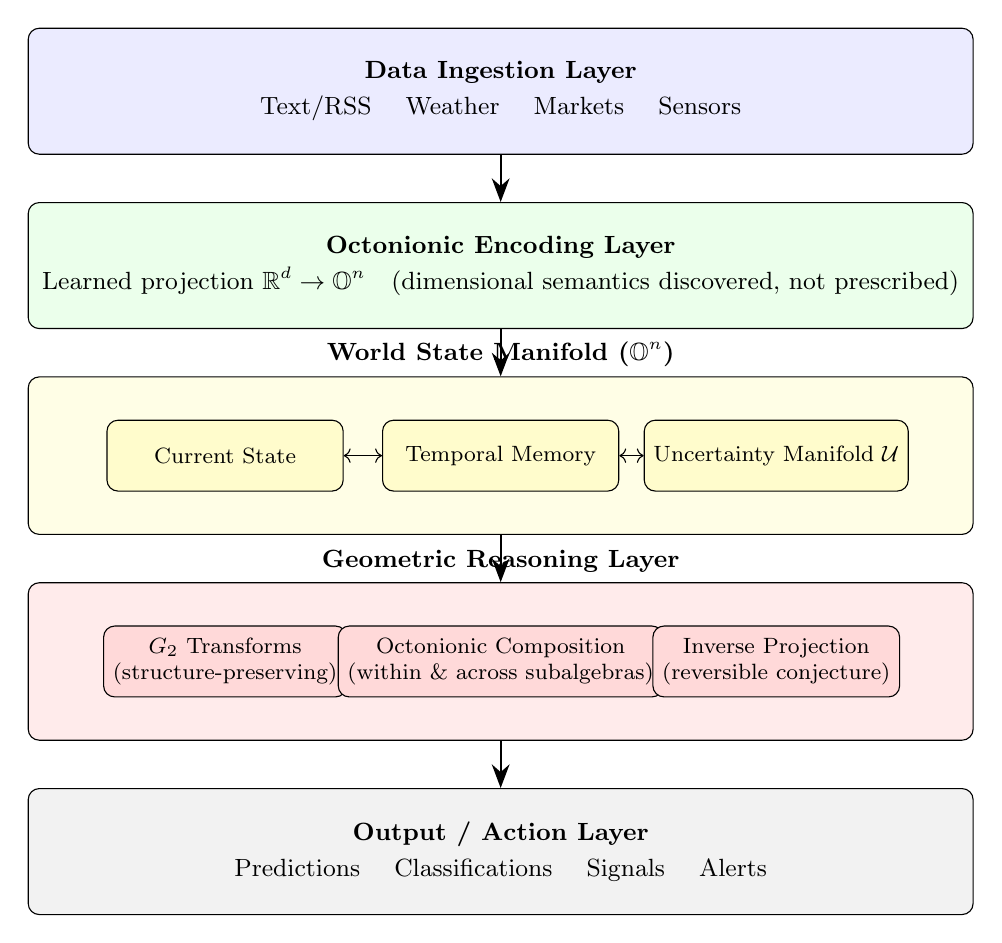
\begin{tikzpicture}[
    layer/.style={draw, rounded corners, minimum width=12cm, minimum height=1.6cm, align=center, font=\small},
    component/.style={draw, rounded corners, minimum width=3cm, minimum height=0.9cm, align=center, font=\footnotesize},
    arrow/.style={-{Stealth[length=3mm]}, thick},
    node distance=0.6cm,
  ]
  % Ingestion
  \node[layer, fill=blue!8] (ingest) {%
    \textbf{Data Ingestion Layer}\\[2pt]
    Text/RSS \quad Weather \quad Markets \quad Sensors};

  % Encoding
  \node[layer, fill=green!8, below=of ingest] (encode) {%
    \textbf{Octonionic Encoding Layer}\\[2pt]
    Learned projection $\Real^d \to \Oct^n$\quad (dimensional semantics discovered, not prescribed)};

  % World state
  \node[layer, fill=yellow!10, below=of encode, minimum height=2cm] (world) {};
  \node[above=0pt] at (world.north) {\small\textbf{World State Manifold ($\Oct^n$)}};
  \node[component, fill=yellow!20] at ($(world.center)+(-3.5,0)$) (cs) {Current State};
  \node[component, fill=yellow!20] at (world.center) (tm) {Temporal Memory};
  \node[component, fill=yellow!20] at ($(world.center)+(3.5,0)$) (um) {Uncertainty Manifold $\mathcal{U}$};
  \draw[<->] (cs) -- (tm);
  \draw[<->] (tm) -- (um);

  % Reasoning
  \node[layer, fill=red!8, below=of world, minimum height=2cm] (reason) {};
  \node[above=0pt] at (reason.north) {\small\textbf{Geometric Reasoning Layer}};
  \node[component, fill=red!15] at ($(reason.center)+(-3.5,0)$) {$G_2$ Transforms\\(structure-preserving)};
  \node[component, fill=red!15] at (reason.center) {Octonionic Composition\\(within \& across subalgebras)};
  \node[component, fill=red!15] at ($(reason.center)+(3.5,0)$) {Inverse Projection\\(reversible conjecture)};

  % Output
  \node[layer, fill=gray!10, below=of reason] (output) {%
    \textbf{Output / Action Layer}\\[2pt]
    Predictions \quad Classifications \quad Signals \quad Alerts};

  % Arrows
  \draw[arrow] (ingest) -- (encode);
  \draw[arrow] (encode) -- (world);
  \draw[arrow] (world) -- (reason);
  \draw[arrow] (reason) -- (output);
\end{tikzpicture}
\caption{High-level architecture of the Octonionic Reasoning Engine (ORE).}
\label{fig:ore-arch}
\end{figure}

\subsection{The Encoding Layer: Learned Octonionic Projection}

The encoding layer maps raw data from heterogeneous streams into~$\Oct^n$, a space of $n$~octonions.

A central design choice is that dimensional semantics are emergent, not assigned. The projection function $\varphi\colon \Real^d \to \Oct^n$ is learned end-to-end, with no prescription that a particular basis element encodes a particular feature. The training process discovers whatever dimensional assignment makes the downstream algebraic operations most effective. This is analogous to how word2vec discovered that vector arithmetic corresponded to semantic relationships, but in a richer algebraic space where the operations have more structure to exploit.

The implementation uses \texttt{OctonionDenseLinear} layers (see \texttt{src/octonion/baselines/\_algebra\_linear.py}) which compute linear maps that respect the octonionic multiplication structure via structure constants:

\begin{lstlisting}[style=python, caption={Octonionic dense linear layer (simplified from codebase).}]
# From src/octonion/baselines/_algebra_linear.py
class OctonionDenseLinear(nn.Module):
    """Linear layer using full octonionic structure constants C[i,j,k]."""
    def forward(self, x: torch.Tensor) -> torch.Tensor:
        # x shape: [batch, in_features, 8]
        # For each (i,j) with nonzero C[i,j,k], compute F.linear
        # on component j, accumulate into output component k
        ...
\end{lstlisting}

\subsection{The World State Manifold}

The world state is a point (or more precisely, a region) in~$\Oct^n$ that evolves continuously as new data arrives.

Temporal memory is maintained by octonionic composition: the new state is formed by multiplying (in the octonionic sense) the current state with the encoded new observation, modulated by learned $G_2$ transformations:
\begin{equation}
W_{t+1} = G(W_t) \cdot \varphi(x_t),
\end{equation}
where $G$ is a learned $G_2$~transformation and $\cdot$ denotes the octonionic product. Because octonionic multiplication is norm-preserving, repeated composition does not cause the state to explode or vanish, a problem that is algebraically impossible with unit octonionic operations.

\subsection{The Reasoning Layer: Geometric Transformations}

Reasoning is performed by sequences of operations falling into three categories:

\textbf{Intra-subalgebra operations} (associative, quaternionic): These operate within one of the 7 quaternionic subalgebras defined by the Fano plane. They are computationally efficient and associative, making gradient computation straightforward.

\textbf{Cross-subalgebra operations} (non-associative, fully octonionic): These mix information across different quaternionic subspaces. The non-associativity means the order of composition matters, and the associator~$[x,y,z]$ measures the magnitude of this order-dependence for a given triple.

\textbf{Inverse projection} (reversible conjecture): Given the current state and an observed output, compute what input state would have produced it. Because all operations are invertible, this is always well-defined. The inverse of the current state is computed via $x^{-1} = \bar{x}/\lvert x \rvert^2$ (see \texttt{src/octonion/\_octonion.py}).

\paragraph{Note on non-associativity and backpropagation.} Standard backpropagation assumes the chain rule, which relies on associativity of function composition. Octonionic operations are non-associative at the algebraic level, but function composition (applying one octonionic operation after another) remains associative at the computational level. The gradient computation is valid; what changes is that the Jacobian of octonionic multiplication has additional structure from the non-commutativity and non-associativity. This is tractable: quaternionic backpropagation has been solved \citep{Parcollet2019}, and the octonionic generalization follows the same pattern with additional terms from the associator. The GHR calculus implementation (see \texttt{src/octonion/calculus/}) validates this approach, demonstrating that correct octonionic gradients match finite-difference approximations to within $10^{-7}$ relative error. Whether this is efficient at scale remains an open empirical question.

\subsection{Multi-Stream Data Ingestion}

The system is designed to ingest heterogeneous real-time data through a unified streaming interface. Different stream types naturally map to different octonionic subspaces during the learned encoding phase. The system discovers which aspects of which streams are ``aligned'' in octonionic space (meaning their octonionic representations compose productively) and which are ``orthogonal'' (carrying independent information).

When signals across multiple streams align geometrically (their octonionic representations reinforce rather than cancel upon composition), the system is detecting a genuine cross-domain pattern. When they do not align, the associator structure characterizes how the signals fail to align, which is itself informative.

This component is planned for Phase~13 of the experimental roadmap (\cref{sec:roadmap}).

%% ====================================================================
\section{Signal Discovery in Streaming Data}
\label{sec:signals}
%% ====================================================================

\subsection{The Geometric Signal Hypothesis}

\textbf{Hypothesis:} In any sufficiently rich data stream, patterns that correspond to genuine causal structure form geometrically coherent structures in octonionic representation space.

This coherence manifests as:
\begin{itemize}[nosep]
  \item \textbf{Norm stability:} True signals, when encoded as octonionic sequences, compose to representations with stable (neither diverging nor collapsing) norms.
  \item \textbf{Subalgebra alignment:} True signals tend to occupy a consistent set of quaternionic subalgebras, meaning their octonionic representations have consistent Fano-plane structure.
  \item \textbf{Associator coherence:} For true signals, the associator $[x,y,z]$ between consecutive observations is small or structured (lying in a low-dimensional submanifold of $\Ima\Oct$). For noise, the associator is large and randomly oriented.
\end{itemize}

\subsection{Noise as Geometric Incoherence}

Noise, by contrast, is characterized by geometric incoherence: random octonionic products distribute uniformly on~$S^7$ without accumulating in any direction; the associator of random triples is generically large and uniformly distributed; noisy sequences do not align with any consistent subalgebra structure.

The world model acts as a geometric filter: it amplifies inputs that are coherent with the learned octonionic structure and attenuates inputs that are not. This is a structural filter (geometrically coherent inputs are integrated; geometrically incoherent inputs are projected to the uncertainty manifold) rather than a threshold filter.

\subsection{Learned Dimensional Semantics}

The system does not preassign meanings to octonionic dimensions. Through training, each dimension (and more importantly, each subalgebra and cross-subalgebra relationship) acquires meaning by virtue of what makes the overall system most effective at its task.

The Fano plane structure plays a central role: the 7 quaternionic subalgebras provide 7 views of the data, each internally associative. The system can learn to assign different semantic roles to different subalgebras. The assignment is discovered during training, not prescribed. The cross-subalgebra (non-associative) interactions capture the relationships between these semantic domains, precisely the kind of cross-domain reasoning that is most challenging for conventional architectures.

%% ====================================================================
\section{Hyperbolic Geometry of the State Space}
\label{sec:hyperbolic}
%% ====================================================================

\subsection{Motivation: Why Flat Geometry is Insufficient}

The architecture described in \cref{sec:architecture} implicitly assumes the world state manifold~$\Oct^n$ carries a flat (Euclidean) metric. This is likely the wrong geometry for knowledge representation, for reasons established independently of the octonionic thesis.

\textbf{Hierarchical structure demands hyperbolic geometry.} Real-world knowledge is hierarchically organized. Trees and DAGs are the natural data structures of knowledge, but trees cannot be embedded in Euclidean space with bounded distortion because the number of nodes at depth~$d$ grows exponentially while the volume of a Euclidean ball grows only polynomially. Hyperbolic space, whose volume grows exponentially with radius, is the natural home for tree-like structures. This has been demonstrated rigorously \citep{Sarkar2011} and applied successfully in ML \citep{Nickel2017,Ganea2018}.

\textbf{Information geometry is naturally hyperbolic.} The Fisher information metric on statistical manifolds is generically hyperbolic. If the octonionic world state encodes something analogous to a distribution over possible world-states, its natural geometry inherits this negative curvature.

\textbf{Scale separation is intrinsic.} In hyperbolic space, distance from the origin has a natural interpretation as level of abstraction. Points near the origin represent general, abstract concepts; points near the boundary represent specific, concrete observations.

\subsection{Three Formulations}

There are at least three distinct ways to combine octonionic algebra with hyperbolic geometry, ranging from pragmatic to exotic.

\subsubsection{Option A: Poincar\'{e} Ball in \texorpdfstring{$\Oct$}{O} (Pragmatic)}

Model the state space as the open unit ball $B^8 = \{ x \in \Oct : \lvert x \rvert < 1 \}$ equipped with the Poincar\'{e} metric:
\begin{equation}
ds^2 = \frac{4\,\lvert dx \rvert^2}{(1 - \lvert x \rvert^2)^2}.
\end{equation}

The key modification is replacing Euclidean operations with their M\"{o}bius gyrovector counterparts. \textbf{Advantage:} well-understood framework with existing tooling. \textbf{Limitation:} the M\"{o}bius operations do not interact cleanly with octonionic multiplication, requiring reconciliation of two separate algebraic structures.

\subsubsection{Option B: Hyperboloid Model via Split Signature (Selected First Approach)}

An octonion has a natural decomposition: 1 real part $+$ 7 imaginary parts. Introducing the Lorentzian inner product:
\begin{equation}
\langle x, y \rangle_L = x_0 y_0 - x_1 y_1 - x_2 y_2 - \cdots - x_7 y_7,
\end{equation}
defines the hyperboloid $H^7 = \{ x \in \Oct : \langle x,x \rangle_L = 1,\; x_0 > 0 \}$ as a model of 7-dimensional hyperbolic space embedded directly in the octonion.

This is compelling because the real/imaginary split of the octonion aligns with the timelike/spacelike split of Minkowski space. Octonionic conjugation $x \mapsto \bar{x}$ flips the sign of the imaginary part, which is precisely the spatial reflection (parity) operation in the Lorentzian picture.

In this formulation, the real part of the octonion encodes the radial position in hyperbolic space, interpretable as the abstraction level or depth in the knowledge hierarchy.

\textbf{Advantage:} The hyperbolic structure is intrinsic to the octonion. \textbf{A tension requiring resolution:} The Lorentzian norm $\langle x,x \rangle_L$ is distinct from the octonionic (Euclidean) norm $\lvert x \rvert^2$. Octonionic multiplication preserves the Euclidean norm, not the Lorentzian one. Consequently, octonionic multiplication moves points off the hyperboloid, necessitating a re-projection step. Whether this re-projection preserves the algebraic properties the architecture depends on (particularly invertibility) requires careful analysis. This is the central open problem of the hyperbolic-octonionic synthesis, addressed experimentally in Phase~12 of the roadmap.

\subsubsection{Option C: The Octonionic Hyperbolic Plane \texorpdfstring{$\Oct H^2$}{OH2} (Exotic)}

The octonionic projective plane $\Oct P^2$ (Cayley plane) is a 16-dimensional Riemannian manifold whose isometry group is the compact exceptional Lie group~$F_4$. Its non-compact dual, $\Oct H^2$, has isometry group~$F_{4(-20)}$ and is a rank-1 symmetric space of non-compact type. Its sectional curvatures range between $-4$ and $-1$ (pinched negative curvature).

This is the most mathematically natural octonionic hyperbolic space, but also the most computationally challenging. The Riemannian exponential and logarithmic maps involve octonionic matrix operations (specifically, operations on $3 \times 3$ Hermitian matrices over~$\Oct$, the Jordan algebra construction).

\begin{epistemicnote}
Option~C is mathematically elegant but may not be computationally tractable for ML training. The machinery of exceptional symmetric spaces is deep and the numerical analysis has not been worked out for gradient-based optimization. This formulation is deferred to future research beyond the current experimental roadmap.
\end{epistemicnote}

\subsection{The Hybrid Hyperboloid-Octonionic Model}

The selected first approach is a modified Option~B that explicitly addresses the Euclidean-vs-Lorentzian tension by separating the algebraic and metric roles of the octonion:
\begin{enumerate}[nosep]
  \item \textbf{Octonionic algebra} governs how states compose: integration of new observations, transformation chaining, and conjecture. These operations use the standard octonionic product with the Euclidean norm.
  \item \textbf{Hyperbolic geometry} governs how states are measured and compared: distances, neighborhoods, gradients, and the loss function.
  \item \textbf{The bridge} between them is a learned projection: after each octonionic composition step, the result is projected back onto the hyperboloid. The projection is parameterized (as a $G_2$-equivariant map) and trained jointly.
\end{enumerate}

\subsection{What Hyperbolic Geometry Contributes to the Architecture}

\textbf{World State Manifold (\cref{sec:architecture}):} The world state lives on $H^{7n}$ (a product of $n$ copies of~$H^7$). Each octonionic component's real part encodes abstraction level. The exponential volume growth provides exponentially more capacity for concrete details than for abstract summaries.

\textbf{The Geometry of Absence (\cref{sec:absence}), formalized:} In hyperbolic space, the boundary at infinity represents the limit of increasingly specific information. The exponential divergence of geodesics means that two directions of missing information that are close at the level of abstract concepts become exponentially separated at the level of specific predictions. The uncertainty manifold acquires a concrete structure:
\begin{equation}
\mathcal{U}(W, \mathcal{C}) \approx \bigl\{ \text{directions in } T_W(H^{7n}) \text{ not constrained by } \mathcal{C} \bigr\}.
\end{equation}

\textbf{Signal Detection (\cref{sec:signals}):} Noise concentrates near the boundary as unstructured high-specificity data, while true signals propagate inward, creating structure at higher levels of abstraction. This radial coherence serves as a distinguisher of genuine patterns from noise.

\textbf{Temporal Memory:} Past observations drift outward in hyperbolic space as they become older. Durable patterns are reinforced at more interior positions. The hyperbolic geometry itself implements a form of episodic-to-semantic memory transition.

\subsection{Connections to Exceptional Structures}

The combination of octonionic algebra and hyperbolic geometry activates several exceptional mathematical structures:

The $3 \times 3$ Hermitian matrices over~$\Oct$ form the exceptional Jordan algebra $J_3(\Oct)$, whose automorphism group is~$F_4$. If the architecture were extended to use these as state representations, the natural symmetry group increases from $G_2$ (14-dim) to $F_4$ (52-dim). The magic square of Freudenthal--Tits constructs the exceptional Lie groups $E_6$, $E_7$, $E_8$ from pairs of division algebras; if the octonionic approach proves fruitful, these structures represent natural extensions for richer geometric models.

\begin{epistemicnote}
The appearance of exceptional Lie groups does not, by itself, validate the approach. Mathematically beautiful systems can be computationally useless. The exceptional structures are a positive signal (suggesting deep mathematical coherence) but not evidence (which requires experiments). The risk of mathematical aesthetics outpacing empirical grounding warrants sustained vigilance.
\end{epistemicnote}

%% ====================================================================
\section{Training and Optimization}
\label{sec:training}
%% ====================================================================

\subsection{The Octonionic Gradient}

Differentiation in non-associative algebras requires care. The key result underlying this work is the \textbf{Generalized Hamilton--Real (GHR) calculus} \citep{Xu2015}, extending the HR calculus (used for quaternionic networks) to octonions. The gradient of a real-valued loss function $L(W)$ with respect to octonionic parameters $W \in \Oct^n$ can be computed as:
\begin{equation}
\frac{\partial L}{\partial W} = \frac{\partial L}{\partial w_0} + \sum_{k=1}^{7} \frac{\partial L}{\partial w_k}\, e_k,
\end{equation}
where each $\partial L / \partial w_k$ is a standard real partial derivative. This is computationally equivalent to treating octonions as~$\Real^8$ for gradient purposes, while the forward pass uses the full octonionic algebraic structure.

The implementation (see \texttt{src/octonion/calculus/\_ghr.py}) uses the Wirtinger-like derivative pair $(\partial f / \partial o,\; \partial f / \partial o^*)$ with a $1/8$ normalization factor (the octonionic extension of the quaternionic~$1/4$). The rotation well-definedness required by the GHR framework is guaranteed by the Moufang identity, which ensures that $\mu \cdot q \cdot \mu^{-1}$ is unambiguous despite non-associativity.

\subsection{Loss Functions for Geometric Reasoning}

The loss function rewards geometric coherence in addition to predictive accuracy. In pseudocode: \pseudocodelabel
\begin{lstlisting}[style=python, caption={ORE loss combining prediction accuracy with geometric regularization (pseudocode).}]
def ore_loss(predicted, actual, world_state, uncertainty_dim,
             w_pred=1.0, w_coherence=0.1, w_uncertainty=0.01, w_invert=0.1):
    loss = w_pred * mse_loss(predicted, actual)
    loss += w_coherence * associator_entropy(world_state)
    loss += w_uncertainty * uncertainty_dim
    loss += w_invert * forward_inverse_roundtrip_error(world_state)
    return loss
\end{lstlisting}

\subsection{\texorpdfstring{$G_2$}{G2}-Equivariant Layers}

To ensure learned transformations respect octonionic structure, they are parameterized as elements of~$G_2$ (or its Lie algebra $\mathfrak{g}_2$). A $G_2$ transformation is specified by 14 parameters (vs.\ 21 for an unconstrained $\SO(7)$ rotation), encoding precisely the algebra-respecting rotations. This is a concrete example of the density argument: 14 parameters yield a transformation that automatically preserves all octonionic structure, while 21 parameters yield an unconstrained rotation that may violate it.

%% ====================================================================
\section{Open Questions and Risks}
\label{sec:risks}
%% ====================================================================

\subsection{Optimization Landscape}

Does octonionic non-associativity create pathological optimization landscapes? The loss surface of an octonionic model may have qualitatively different properties from real-valued or quaternionic models. Artin's theorem guarantees that any two octonions generate an associative subalgebra, so pairwise interactions are well-behaved; pathology can only arise from three-way or higher interactions. Phase~5 of the experimental roadmap addresses this question empirically and serves as a go/no-go gate.

\subsection{Scaling Behavior}

How does representational density scale with model size? The $14/8 = 1.75$ density ratio (\cref{sec:density}) is computed for a single octonion. Whether this ratio is maintained, improved, or degraded when scaling to~$\Oct^n$ for large~$n$ remains unclear.

\subsection{Numerical Stability}

Is octonionic computation numerically stable in finite-precision arithmetic? The non-associativity means that $(xy)z$ and $x(yz)$ give genuinely different results, even in exact arithmetic. In floating-point, the rounding behavior of these two groupings differs. The \texttt{StabilizingNorm} module (see \texttt{src/octonion/baselines/\_stabilization.py}) extends stable depth by 2.5--5$\times$ depending on the algebra.

\subsection{The ``Why Not \texorpdfstring{$\Real^8$}{R8}?'' Challenge}

Can a sufficiently large real-valued model learn the same representations? The universal approximation theorem guarantees that a large enough real-valued network can approximate any function. The octonionic claim is not that $\Real^8$ cannot learn what~$\Oct$ encodes, but that~$\Oct$ provides sufficient inductive bias that the octonionic model will learn faster, with fewer parameters, and with better generalization. The experimental design includes an $\Real^8$ dense mixing baseline in every comparison (see \texttt{src/octonion/baselines/\_dense\_mixing.py}).

\subsection{The Non-Associativity Trade-off}

Is non-associativity a feature or a limitation? This work argues it is a feature (encoding context-dependence and richer geometry), but certain standard architectural patterns require rethinking. The computational overhead of tracking parenthesization in deep networks may offset the representational advantage.

\subsection{Grounding the Geometry of Absence}

Is the uncertainty manifold concept formally well-defined and computable? The description in \cref{sec:absence} requires completion: how is the constraint set $\mathcal{C}$ defined? Is $\mathcal{U}(W, \mathcal{C})$ a smooth manifold or something more pathological? Can its geometry be efficiently computed? Phase~10 of the experimental roadmap tests this empirically.

\subsection{The Hyperboloid Projection Problem}

Does re-projection onto the hyperboloid after octonionic multiplication destroy the algebraic properties required by the architecture? This is the central open problem of \cref{sec:hyperbolic}. The projection preserves imaginary direction but recomputes the real part, meaning the real part becomes determined by the imaginary parts. Phase~12 of the experimental roadmap is dedicated to this characterization.

\subsection{Numerical Stability in Hyperbolic Space}

Do hyperbolic coordinates amplify floating-point issues? Hyperbolic space is challenging for floating-point arithmetic: $\cosh$ and $\sinh$ grow exponentially, while the Poincar\'{e} ball model requires exponentially fine precision near the boundary. Both issues are documented in the hyperbolic ML literature and have engineering solutions (logarithmic coordinates, mixed-precision arithmetic), but their interaction with octonionic computation has not been studied.

%% ====================================================================
\section{Experimental Roadmap}
\label{sec:roadmap}
%% ====================================================================

The experimental program proceeds bottom-up, validating each theoretical claim with controlled experiments before building on it. All experiments use Python with PyTorch and ROCm acceleration on AMD GPU hardware.

\begin{description}[style=nextline, leftmargin=1em]
  \item[Phase 1: Octonionic Algebra]
  Implement and rigorously test the core octonionic algebra library. Verify Moufang identities on 10,000+ random triples, norm preservation to $10^{-12}$, Cayley--Dickson/Fano cross-check, inverse correctness, and alternativity. \emph{Complete.}

  \item[Phase 2: GHR Calculus]
  Implement octonionic backpropagation via GHR Wirtinger formalism. Verify gradients match finite-difference to $10^{-5}$ on single-layer and 5-layer compositions with mixed parenthesization. Demonstrate that naive chain rule produces incorrect gradients. \emph{Complete.}

  \item[Phase 3: Baseline Implementations]
  Build fair comparison networks for R, C, H, O with matched parameter counts ($<1\%$ deviation), identical architecture skeleton, and algebra-specific batch normalization. \emph{Complete.}

  \item[Phase 4: Numerical Stability]
  Characterize precision degradation across depths (10, 50, 100, 500 layers), measure condition numbers, compare float32 vs.\ float64, and validate mitigation strategies. \emph{Complete.}

  \item[Phase 5: Optimization Landscape (Go/No-Go Gate)]
  Characterize gradient variance across 20+ seeds, Hessian eigenspectrum at convergence, convergence profiles across 3+ optimizers, and determine whether octonionic networks converge to solutions within $2\times$ loss of $\Real^8$ baseline. \emph{Experiments running.}

  \item[Phase 6: Reversibility Claim]
  Test algebraic inversion quality vs.\ RevNet/INN baselines on synthetic tasks with known forward models and ground-truth inverses.

  \item[Phase 7: Density and Geometric Claims]
  Run matched-parameter density comparisons across R/C/H/O on 3+ tasks with statistical significance testing. Include $\Real^8$ dense mixing baseline in every comparison.

  \item[Phase 8: $G_2$ Equivariance and Hyperbolic Hybrid]
  Implement $G_2$-equivariant layers and verify numerical equivariance. Implement the hyperboloid-octonionic hybrid model (Option~B). Test on hierarchical data against Poincar\'{e} embedding baselines.

  \item[Phase 9: Associator and Subalgebra Analysis]
  Build associator-aware architectures that use $[a,b,c]$ as an attention, regularization, or gating signal. Decompose trained representations along the 7 Fano plane subalgebras to test for specialization.

  \item[Phase 10: Predict-and-Fill Benchmarks]
  Validate the geometry of absence through predict-and-fill tasks requiring the model to identify missing data dimensions and generate plausible completions via inverse projection.

  \item[Phase 11: Applied Single-Stream Benchmarks]
  Test octonionic representations on anomaly detection and time series prediction, comparing against LSTM and Transformer baselines with matched parameter counts.

  \item[Phase 12: Hyperboloid Projection Stability]
  Characterize the Euclidean--Lorentzian projection distortion: measure $\lvert \mathrm{project}(a \cdot b) - \mathrm{project}(a) \ast_H \mathrm{project}(b) \rvert$ for random and structured inputs. Quantify invertibility degradation after repeated re-projection.

  \item[Phase 13: Multi-Stream Data Fusion]
  Build an ORE proof-of-concept ingesting 3+ heterogeneous data streams. Validate cross-stream geometric signal detection. Analyze Fano plane subalgebra specialization across stream types.
\end{description}

%% ====================================================================
\section{Conclusion}
\label{sec:conclusion}
%% ====================================================================

The octonionic reasoning engine sits at the intersection of abstract algebra, differential geometry, and machine learning. The mathematical arguments supporting this approach are:

\begin{enumerate}
  \item \textbf{Hurwitz's theorem provides a hard ceiling.} Octonions are the last normed division algebra. If the program of using richer algebras for richer representations is viable, it terminates here.

  \item \textbf{The density ratio is unique.} No other algebra achieves an automorphism-to-dimension ratio above~1; octonions achieve~1.75.

  \item \textbf{Invertibility is algebraically guaranteed.} Every non-zero octonion has a unique inverse, enabling reversible reasoning without architectural constraints.

  \item \textbf{The Fano plane provides natural multi-view decomposition.} Seven overlapping quaternionic subalgebras give the model 7 internally-associative perspectives on its data, with non-associative cross-talk encoding context-dependence.

  \item \textbf{Non-associativity encodes order-dependence.} The associator $[a,b,c] = (ab)c - a(bc)$ measures a fundamental truth: the order and grouping of reasoning steps matters. The difference between groupings is itself an informative geometric signal.
\end{enumerate}

Whether these mathematical properties translate into practical ML advantages is an empirical question. This thesis provides the theoretical foundation and architectural blueprint; the experimental roadmap (\cref{sec:roadmap}) charts the path to evidence.

%% ====================================================================
\bibliographystyle{plainnat}
\bibliography{references}

%% ====================================================================
\appendix

\section{The Fano Plane}
\label{app:fano}

The Fano plane is the finite projective plane $\PG(2,2)$, encoding the octonionic multiplication table. It has 7 points (corresponding to the imaginary basis units $e_1$ through $e_7$) and 7 lines (including one inscribed circle).

\begin{figure}[ht]
\centering
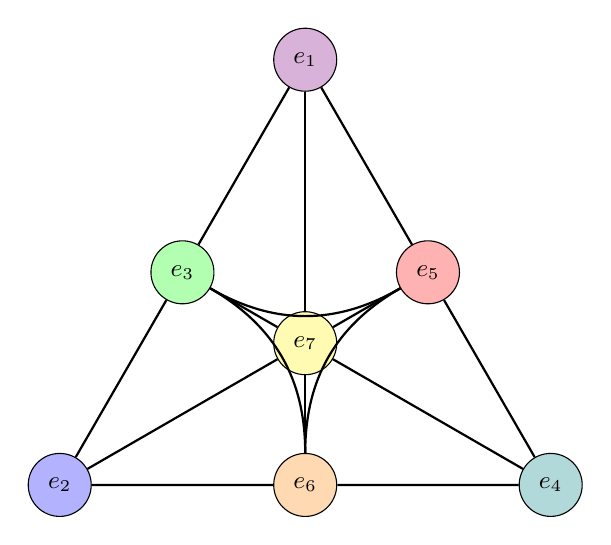
\begin{tikzpicture}[
    vertex/.style={circle, draw, fill=#1!30, minimum size=8mm, inner sep=0pt, font=\small\bfseries},
    vertex/.default=blue,
    edge/.style={thick},
    scale=1.8,
  ]
  % Triangle vertices
  \node[vertex=violet]  (e1) at (90:2)    {$e_1$};
  \node[vertex=blue]    (e2) at (210:2)   {$e_2$};
  \node[vertex=teal]    (e4) at (330:2)   {$e_4$};

  % Midpoints of triangle edges
  \node[vertex=green]   (e3) at ($(e1)!0.5!(e2)$)  {$e_3$};
  \node[vertex=red]     (e5) at ($(e1)!0.5!(e4)$)  {$e_5$};
  \node[vertex=orange]  (e6) at ($(e2)!0.5!(e4)$)  {$e_6$};

  % Center
  \node[vertex=yellow]  (e7) at (0,0)     {$e_7$};

  % Triangle edges (3 lines of the Fano plane)
  \draw[edge] (e1) -- (e3) -- (e2);
  \draw[edge] (e1) -- (e5) -- (e4);
  \draw[edge] (e2) -- (e6) -- (e4);

  % Medians (3 lines through center)
  \draw[edge] (e3) -- (e7) -- (e4);
  \draw[edge] (e5) -- (e7) -- (e2);
  \draw[edge] (e6) -- (e7) -- (e1);

  % Inscribed circle (the 7th line)
  \draw[edge] (e3) to[bend right=30] (e5);
  \draw[edge] (e5) to[bend right=30] (e6);
  \draw[edge] (e6) to[bend right=30] (e3);
\end{tikzpicture}
\caption{The Fano plane. The 7 lines are: $(1,2,3)$, $(1,4,5)$, $(1,7,6)$, $(2,4,6)$, $(2,5,7)$, $(3,4,7)$, $(3,6,5)$. Each line defines a quaternionic subalgebra: $e_i \cdot e_j = e_k$ (oriented cyclically). Anti-cyclic products carry a negative sign: $e_j \cdot e_i = -e_k$.}
\label{fig:fano}
\end{figure}

Each imaginary unit belongs to exactly 3 of the 7 subalgebras, and any two imaginary units share exactly 1 subalgebra (in which their product is associative). Non-associativity arises only when three imaginary units span more than one subalgebra.

\section{\texorpdfstring{$G_2$}{G2} as a Subgroup of \texorpdfstring{$\SO(7)$}{SO(7)}}
\label{app:g2}

$G_2$ is the stabilizer of the 3-form:
\begin{equation}
\omega = e^{123} + e^{145} + e^{176} + e^{246} + e^{257} + e^{347} + e^{365},
\end{equation}
where $e^{ijk} = e^i \wedge e^j \wedge e^k$ are basis 3-forms on~$\Real^7$ (the imaginary octonions). This 3-form encodes the entire octonionic multiplication table: preserving it is equivalent to preserving the octonionic algebra structure.

$G_2$ has 14 generators ($= \dim\SO(7) - 7$ constraints from~$\omega$), and every $G_2$ element is an $\SO(7)$ rotation that additionally preserves the cross product on $\Ima\Oct$.

\end{document}
